
%%% Local Variables:
%%% mode: latex
%%% TeX-master: t
%%% End:

\chapter{标签化地址空间}
\label{chap:labeladdrspace}

虚拟地址空间对应多进程场景,随着单节点计算能力的增强以及云计算场景发展,
多租户场景成为一种趋势。

虚拟机抽象的出现是应对这下趋势的一个变化,将一台物理机隔离为多个无关的虚拟机,
现在虚拟机基于的硬件技术包括:内存划分技术EPT、I/O虚拟化I/O-MMU、MSI中断等。
这些技术在Hypervisor的支持下协同工作,向上层展现出虚拟的隔离计算机。

但这里的隔离并非真正的隔离,多个虚拟机仍然通Hypervisor实现对共享硬件资源的使用,
如hypervisor需要对页表寄存器进行控制,实现地址空间的切换;
通过对I/O设备的代理访问,实现虚拟I/O设备;

标签化地址空间的目的是将多个虚拟机真正的物理隔离开。


为了适应当前多应用以及多租户的使用场景,计算机系统软件栈在不断发展。
以Linux操作系统为例,其包含多级嵌套结构以适应于不同的应用场景,如图\ref{}所示。
操作系统最小的调度单元是线程,多个线程运行在同一个进程的地址空间中,
线程之间共享全部的软硬件资源;
不同的进程具有独立的虚拟地址空间,它们之间共享除用户地址空间外的全部软硬件资源,
如操作系统内核;
进程包含在名字空间中,一个操作系统中可同时存在多个名字空间,
它们拥有自己的PID、网络、根文件系统,名字空间只共享部分操作系统内核,硬件依然是全共享;
在Linux操作系统的最顶层是虚拟机,每个虚拟机都运行自己的操作系统,
在操作系统及以上层次不存在共享,虚拟机之间通过Hypervisor共享硬件资源。


%%
%%Why we need PARD? => single/batch-program change to multi-thread program to multi-tent/cloud
%%但体系结构几乎没有变化,不能区分不同应用,造成\ref{chap02}中的一些问题。
%%随着核数增多,单个应用无法用满所有的核,出现了虚拟化技术,其本质是在虚拟地址空间之外增加一层地址空间
%%本章介绍PARD体系结构与其基本特性,对比PARD与SDN结构,PARD系统使用实例,如何在现有系统中构造出PARD。
%%% Need of a PARD's labeled address space
%%\section{标签化地址空间}
%%%软件层标签化(cgroup/VM),逻辑域,
%%%标签化用途
%%%如何实现
%%多个虚拟地址空间对应一个物理地址空间。
%%EPT增加了一级地址映射,实现内存划分;I/O MMU技术让硬件设备能够识别EPT增加的一级地址空间。
%%PCI-E的SR-IOV技术让设备
%%

\section{相关工作}

体系结构对应用区分的支持,从最早的虚拟地址空间,到虚拟化支持。
本节将从资源隔离与性能隔离两个方面介绍应用区分的相关工作。

\subsection{资源隔离}

最早被隔离的资源是CPU,通过保存寄存器状态,并在进程切换时切换寄存器,实现CPU资源共享。
随着内存需求的增加,虚拟内存出现,实现用户地址空间的隔离。
虚拟化的出现,对虚拟机访存性能提出需求,体系结构也做出了相应的更改。
以Intel为例,为更好的支持虚拟化环境,其VMX技术增加了VCPU抽象,

单一地址空间 => 虚拟内存(多地址空间,保护)=> 虚拟化,tagged-TLB,VT技术,多租户
                                            => 容器技术
对计算机的使用趋势是从单一应用到多应用,

\subsection{性能区分}

\subsubsection*{Intel Resource Director Technology(RDT)技术}

针对多处理器芯片中多应用共享的特征,Intel提出了Resource Director Technology方案来解决多应用资源共享冲突问题。
如图\ref{fig:intel-rdt-overview}所示,该方案的硬件基础是资源监控与资源分配控制机制,
同时提供基于"监控->策略->控制"组合的闭环方式来实现应用感知的资源管理框架。
其中资源监控提高了资源使用情况的能见度,使得资源利用率可以被跟踪,同时可以侦测到应用性能随资源的变化,
为上层的资源调度提供数据基础;
而硬件支持的资源分配控制机制,使得上层软件可以控制对硬件共享资源的使用。

% Intel RDT Overview
\begin{figure}[H]
  \centering
  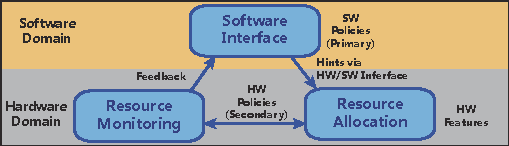
\includegraphics{x86eval/intel-rdt-overview}
  \caption[Intel Resource Director Technology (RDT) 技术示意图]{
    Intel Resource Director Technology (RDT)技术:硬件提供资源监控与分配功能,
    软件负责对资源使用进行调度,实现资源按需求动态分配。}
  \label{fig:intel-rdt-overview}
\end{figure}

目前Intel已经将RDT方案应用到共享末级缓存和内存控制器中,通过CMT/MBM技术实现对缓存容量
以及内存带宽的监控;通过CAT技术实现对缓存容量划分的支持。

CMT和MBM技术允许操作系统或Hypervisor/VMM监控在其上运行的应用对共享缓存与内存带宽
的使用情况,图\ref{fig:intel-cmt-flow}是该技术的流程示意图。
操作系统或VMM首先为执行实体(如线程、进程或虚拟机)分配资源编号RMID,后续的监控结果都将
以RMID的形式进行汇报。在OS/VMM执行调度并进行上下文切换时,将被调度实体的的RMID写入到目标
处理器核对应的寄存器中。OS/VMM可以随时通过RMID查询各个执行实体的资源使用情况,如共享缓存
占用或访存带宽等信息。
 
% Intel CMT Flow
\begin{figure}[H]
  \centering
  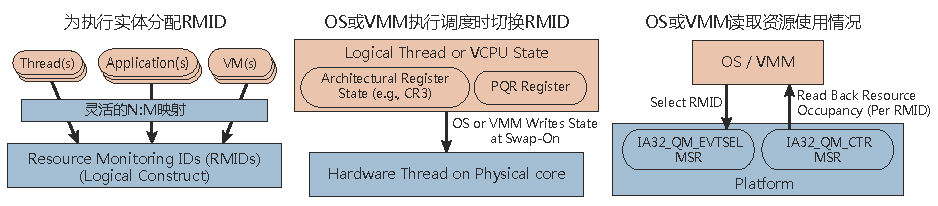
\includegraphics{x86eval/intel-cmt-flow}
  \caption[Intel Cache Monitor Technology (CMT) 技术流程]{Intel CMT技术流程:
   (1)为线程、应用或虚拟机等执行实体分配资源编号RMID;(2)将包含RMID的PQR寄存器
   保存在线程TCB或虚拟机VCPU中,并在执行上下文切换时写入到处理器核对应的物理寄存器中;
   (3)根据RMID使用MSRs寄存器获取共享资源使用情况。}
%Threads, applications, VMs or any combination can be associated with an RMID, enabling very flexible monitoring. As an example, all threads in a VM could be given the same RMID for simple per-VM monitoring. (2) The PQR register (containing an RMID) stored as part of a thread or VCPU state, which is written onto the thread-specific registers when a software thread is scheduled on a hardware thread for execution. (3) After a period of time (as defined by the software) the occupancy data for a given RMID can be read back through a pair of keyhole MSRs which provide the ability to input an RMID and Event ID (EvtID) in a selection MSR, and the hardware retrieves and returns the occupancy in the data MSR.}
  \label{fig:intel-cmt-flow}
\end{figure}

CAT技术为OS/VMM提供了控制末级共享缓存容量的功能,如图\ref{fig:intel-cat-flow}所示,
当该功能被开启后,应用将只能使用分配给它的Cache容量,实现路划分。
路划分策略是以COS为粒度进行指定,OS/VMM首先为某一COS制定路划分策略,并将该COS关联到使用
该策略的执行实体中,并在上下文划分时将被调度实体的COS写入到处理器核对应的寄存器中,
共享缓存根据COS对应的策略来进行缓存替换操作。

\begin{figure}[H]
  \centering
  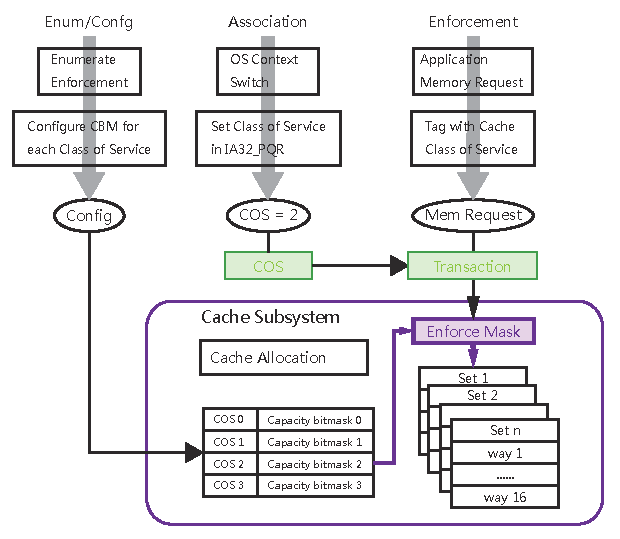
\includegraphics[height=8cm]{x86eval/intel-cat-flow}
  \caption[Intel Cache Allocation Technology (CAT) 技术流程]{Intel CAT技术流程}
  \label{fig:intel-cat-flow}
\end{figure}






\section{标签与隔离粒度}

如何划分地址空间:虚拟机、容器、进程、etc...

\section{标签机制实现}

\subsection{标签的传播}

不同总线上如何实现地址空间

\subsubsection{通过标签实现内存地址空间隔离}

地址映射位置,与EPT技术对比

Cache一致性场景下如何实现标签化地址空间

处理器核共享场景(0.1个处理器核)

\subsubsection{通过标签实现I/O地址空间隔离}

SR-IOV or pseudoMR-IOV

\section{体系结构的可行性}

在X86或ARM上实现该架构

%如何在一个ARM中实现PARD功能

如上节所述,PARD并不是一个完全全新的体系结构,而是对现有体系结构的扩展。
为了说明如何将PARD扩展到一个现有的体系结构中,本节首先构建了一台虚拟计算机,
我们将其命名为XXXX,如图\ref{fig:XXX-computer}所示。
XXX包含两路4核的处理器,每个处理器核拥有独立的一级缓存L1-I和L1-D,
每个Socket的四个处理器核共享一个16路2MB的二级缓存;
两个Socket拥有自己的内存控制器,同时使用MESI目录协议实现NUMA内存访问;
XXX的I/O子系统包含SATA控制器和两个以太网卡,通过IOH芯片与两个处理器相连。
XXX的结构可以很好的匹配到目前流行体系结构中(如X86或ARM)。

\subsection{Computer as a Network => PARD}

\subsection{像SDN一样集中式的管理计算机}

\section{PARD与SDN}

在第\ref{chap:intro}章中我们提出
同时,计算机内部也可以被看做一个网络,如图\ref{fig:computer-as-a-network}所示,
CPU核、共享缓存、内存控制器、I/O设备等可以被看做是网络节点;除了处理请求以外,
这些“网络节点”与网络中的路由器/交换机具有相似的请求转发功能;
而它们之间也通过包进行通信,如:片内通信使用NoC包,片间通信的QPI/HT包,
以及I/O部分使用的PCI-E包。
将网络领域的区分化服务和软件定义网络的思想应用到计算机内部的网络,
用以解决数据中心当前面临的资源利用率与应用服务质量矛盾,是本文的主要研究思路与动机。

与在网络中部署SDN相比,在计算机体系结构“网络”中部署SDN会面临以下三个挑战:

首先,在整个网络栈中EndPoint是唯一的请求来源,因此SDN可以很容易的将标签机制实现在网络栈中;
与之相对的,在计算机体系结构中存在大量的硬件部件都能够发送请求,而这些请求类型又不尽相同,
因此在这样的环境下如何为请求打上标签是一个很大的挑战。

其次,在网络中所有的交换机都执行相同的存储/转发(store-and-forward)操作,但在计算机内部
不同的部件都有不同的功能,而不只是简单的存储/转发,如何为这些不同类型的部件(如末级缓存控制器、
内存控制器、I/O设备等)设计统一的控制面结构是另一个挑战。

最后,在网络交换机中已经包含了一个firmware固件用于访问和配置交换机的控制面,但计算机中却缺少
这样的firmware。现有的IPMI只被用来做有限的监控与管理功能,如对温度、风扇转速和电源控制。
因此,需要在计算机内部提供一种这样的部件实现与其它众多的控制面的通信与管理,并提供一个灵活的
编程接口对这些控制面进行操作。


